\section{CCTF Resilient Server}
\label{sec:cctf-resilient}

\subsection{Scenario}
\label{sec:cctf-resilient:scenario}

%\autoref{fig:cctf-network} shows the network provided as an integral part of both the Resilient Server and Secure Server CCTFs. 

The \textit{red team} (or \textit{attacking team}) had control over the three clients shown on the right of \autoref{fig:cctf-network}. Instead, the \textit{blue team} (or \textit{defending team}) managed the \textit{server} and the \textit{gateway}.

The \textit{server}'s only function was to provide ten static HTML pages while the \textit{gateway} acted as a middleman between the server and the router (external network). 
On the other side of the \textit{router}, the three \textit{client}s were free to cause Denial of Service (\textit{DoS}) to the server. The only requirement was that one of them had to behave as a legitimate user, performing not more than one request per second.

The \textit{router} was not accessible by any team, and the Teaching Assistant (\textit{TA}) controlled it. The operative system of all the machines was Ubuntu 18.04. Moreover, the testbed was isolated from the external network, with packages updates (\texttt{apt}) provided through a local repository.

The rules prohibited us from using the interfaces or the IPs of the DETERLab network. Both defense and attack were allowed only using the testbed interfaces and IPs shown in \autoref{fig:cctf-network}, which were the same for both the red and the blue team  \cite{resilient-server}. Attachment \ref{sec:attachments:networks} shows a complete list of the networks available in the experiment.

\begin{figure}[ht]
    \centering
    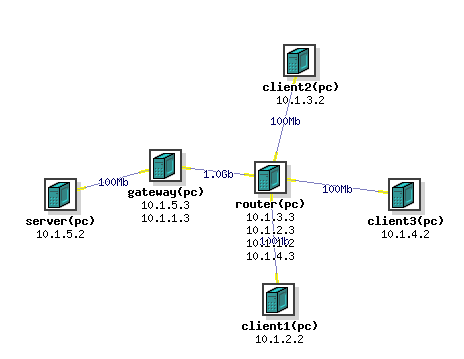
\includegraphics[width=0.6\textwidth]{drawable/network.png}
    \captionsetup{justification=centering}
    \caption{The full network diagram with interface IPs.\\DETERLab management interfaces are not shown.}
    \label{fig:cctf-network}
\end{figure}

\subsection{Environment setup}
\label{sec:cctf-resilient:env-setup}

We started the preparation phase by setting up a private GitHub repository containing all the tools, scripts, and materials needed for the CCTF. 

Each member of the group cloned the repository on their DETERLab home directory, which is mounted as a Network File System (\textit{NFS}) drive on the \texttt{users.deterlab.net} machine along with all the experiment machines.

To automate the setup process, we wrote bootstrap scripts that pulled and installed dependencies automatically and configured the machines accordingly. For the \textit{gateway} and the \textit{server} they mainly set up the firewall rules and configured the web server. For the \textit{clients}, the script installed the few tools that were not already available on the repository.


\subsection{Attack preparation}
\label{sec:cctf-resilient:att-prep}

\subsubsection{Goals}
\label{sec:cctf-resilient:att-prep:goals}

The red team had the following tasks:

\begin{itemize}
    \item At the beginning, choose a client and declare it as ``legitimate'' to the Teaching Assistant, then set it up to act legitimately\footnote{``Legitimately'' means a minimum of one request every ten seconds and a maximum of one every second.}.
    \item Use the remaining two clients to disrupt the web server's Service Level Agreement by making it exhaust its resources, flood incoming links, and ultimately cause it to crash and be unable to serve any request.
\end{itemize}

\subsubsection{Tools used}
\label{sec:cctf-resilient:att-prep:tools-used}

To organize the attack, we spent a lot of time looking for open source tools that could allow us to cause DoS to the blue team machines. One of the problems in this phase was the lack of a WAN connection in the testbed. While we were able to retrieve and update some packages using the local \texttt{apt} repository, we could not use tools like \textit{pip} nor download anything directly to the machines. 
We partially solved this issue by fetching the source code of some tools along with their dependencies and compiling everything locally.

After discarding various ineffective or useless tools, we narrowed down our list to the following ones: 

\begin{itemize}
    \item \texttt{GoldenEye}~\cite{github:goldeneye}: GoldenEye is a now-deprecated, yet-useful open-source tool that employs maximum parallelism and sets up a customizable amount of threads and outbound sockets on the machine. These sockets repeatedly start pinging the target while abusing the HTTP Keep-Alive options to keep connections open and waste the target's memory. Its downside is that it is nearly impossible to stop.
    \item \texttt{Hulk}~\cite{github:hulk}: Hulk is a Go/Python tool that spawns several threads for each connection and stresses the target server by repeatedly making concurrent \texttt{HTTP} requests and leaving the connections open, exhausting its resource pool.
    \item \texttt{SlowLoris}~\cite{github:slowloris}: SlowLoris is a DoS tool that starts making a slew of parallel requests to the target server. Once the connections are open, it sends headers periodically to keep them alive, thus exhausting the servers' thread pool and memory and bringing it to a halt.
    \item \texttt{Sockstress}~\cite{github:sockstress}: a slightly different implementation of the SlowLoris tool. It not only keeps an empty connection open, but It also allows requesting arbitrary pages from a web server.
    \item \texttt{Targa3}~\cite{github:etccetera}: a simple C program that generates packets with weird combinations of \texttt{TCP} and \texttt{IP} flags (e.g., invalid fragmentation, packet size, offsets, \texttt{TCP} segments) and starts flooding the target server with them.
    \item \texttt{hping3}~\cite{linux-die:hping3}: 
    a versatile Unix tool that allows elaborate packet crafting. It handles fragmentation, arbitrary packet body, and size. It also supports spoofing and can be used as a DoS tool, albeit with limitations. 
\end{itemize}

An honorable mention goes to \texttt{loacker}. While testing \texttt{hping3}'s capabilities, we noticed that it was not good enough. Since our goal was to obfuscate the \texttt{SYN} flood, we wanted to craft packets and make them look like \texttt{SYN} packets of \texttt{curl} requests. Even if very flexible, \texttt{hping3} did not support setting TCP options such as \texttt{sack-permitted} or \texttt{NOP}. 
To overcome this limit, we built \texttt{loacker}: a small Go program, which employs maximum parallelism and uses raw sockets to flood the target with credible, \texttt{curl}-like \texttt{SYN} packets, and that also allows for source IP spoofing.

We developed our tool to generate legitimate requests, merely called \texttt{legitimate}. It is a small \texttt{bash} script that continuously sends \texttt{curl} requests to the server while logging parameters such as response times and error codes. It also has an option to modify the random delay between requests.

\subsubsection{Strategy overview}
\label{sec:cctf-resilient:att-prep:strat-out}

Before starting the CCTF, we outlined a four-part strategy, hoping to have a flexible and structured template that would allow us to focus our efforts on each phase, rather than just sending random attacks hoping for something to work.

\begin{itemize}
    \item \textbf{Reconnaissance}: enumerate the vulnerabilities of the adversary team by checking their open ports, firewall rules, and the blueprint of the authorized traffic.
    \item \textbf{Focus}: after discovering the enemy team's configuration and key weaknesses (e.g., some bogus TCP combinations were allowed), choose the best attack plan.
    \item \textbf{Slow start}: to avoid wasting all of our options immediately, start attacking the enemy team with our weaker tools -- in the hope that some misconfiguration could give us an early advantage.
    \item \textbf{Wafer attack}: launch our most powerful tools (\texttt{loacker} and \texttt{hping3}), hoping to catch the defending team unprepared and unable to respond to the attack promptly.
\end{itemize}

\subsection{Defense preparation}
\label{sec:cctf-resilient:def-prep}

\subsubsection{Goals}
\label{sec:cctf-resilient:def-prep:goals}

The blue team only goal was to keep the server response time below 500 milliseconds (ms).
As already mentioned in \autoref{sec:cctf-resilient:scenario}, the web server had to provide ten static HTML pages, numbered from 1 to 10 and customized at the team's will. 

\subsubsection{Strategy overview}
\label{sec:cctf-resilient:def-prep:strat-out}

The defense strategy involved TCP/IP stack hardening on both server and gateway, installing Varnish \cite{varnish}, and configuring a two-level firewall.
Moreover, we built ad hoc monitoring tools to examine the incoming network traffic.

\paragraph{Gateway}
\label{sec:cctf-resilient:def-prep:gateway}

As the gateway was our first level of defense, we wanted to set up the firewall to block most of the unwanted traffic efficiently.

We used the \texttt{PREROUTING} chain of the \texttt{raw} and \texttt{mangle} tables to do this, both configured with a default \texttt{ACCEPT} policy. Instead, we set up a default \texttt{DROP} policy for the \texttt{INPUT}, \texttt{FORWARD}, and \texttt{OUTPUT} chains.

The \texttt{raw} table filtering happened before connection tracking (CONNTRACK), making it less CPU intensive.
We used it to filter out fragmented packets, bogus TCP flags, unusual Maximum Segment Size (MSS)\footnote{The typical MSS of an IPv4 packet is usually 1460 bytes~\cite{kurose-ross}} values in \texttt{SYN} packets, UDP and ICMP protocols. Moreover, we added an IP whitelist with the known IPs of the whole network.

The \texttt{mangle} table filtering happened after the connection tracking, allowing us to implement a stateful firewall. We used it to block \texttt{INVALID} packets, and new connections started with packets without the \texttt{SYN} flag.

In the \texttt{INPUT} and \texttt{OUTPUT} chains, we blocked almost everything that was coming from and going to the router -- connections with the server or DETERLab were left untouched -- while on the \texttt{FORWARD} chain, we allowed only TCP traffic directed to the server on port 80.

Finally, we tweaked the TCP/IP stack. These settings are directly tied to the Linux kernel but can be changed at runtime. In particular, we increased memory allocation and the size of the \texttt{SYN} backlog, we reduced the number of \texttt{SYN}-\texttt{ACK} retries and the \texttt{FIN} timeout, and we switched the congestion control algorithm to BBR~\cite{bbr}. The \texttt{SYN} cookies were already enabled by default.

\paragraph{Server}
\label{sec:cctf-resilient:def-prep:server}

On the server, we configured the firewall using only the \texttt{INPUT} and \texttt{OUTPUT} chains of \texttt{iptables}, with a default \texttt{DROP} policy. Additionally, we allowed bidirectional TCP traffic on port 80 only for \texttt{ESTABLISHED} and \texttt{RELATED} connections.

We hardened the TCP/IP stack in the server the same way we did in the gateway.

Then we installed Varnish in front of Apache web server. Varnish is a web application accelerator, or HTTP reverse proxy, that caches the contents and serves them at a much higher rate~\cite{varnish}. As the web server was serving only static (empty) HTML pages, it was more efficient than \textit{Apache}, easier to set up than \textit{Nginx}, and it could handle slow HTTP attacks better.

We also configured Varnish as an application-level firewall, filtering out unwanted HTTP requests and allowing only GET requests.

\paragraph{Monitoring}
\label{sec:cctf-resilient:def-prep:monitoring}

We spent a lot of time developing monitoring tools. We wanted something capable of providing useful insight into the actions taken by the \textit{red team} and an easy way to check the server status constantly. 

After analyzing different scenarios, we depicted three tools, and we wrote them using Python and relying on the Pyshark~\cite{github:pyshark} library.

\begin{itemize}
    \item \texttt{traffic\_logger.py}: constantly checked the incoming traffic, displaying and updating every 500 ms a table with type, source IP, and size of each packet received. It was running on both the server and the gateway, helping us clearly understand what was happening on the network and understand what the red team was doing. \autoref{tab:traffic_logger} schematizes the script's output.
    \begin{table}[ht]
        \centering
        \begin{tabular}{|c|c|c|c|c|c|c|c|c|c|c|}
            \hline
            \texttt{SRC\_IP} & \texttt{TCP} & \texttt{B\_TCP} & \texttt{SYN} & \texttt{B\_SYN} & \texttt{UDP} & \texttt{B\_UDP} & \texttt{ICMP} & \texttt{B\_ICMP} & \texttt{OTHER} & \texttt{B\_OTHER} \\
            \hline
            \texttt{CLIENT\_1} & \texttt{0} & \texttt{0} & \texttt{0} & \texttt{0} & \texttt{0} & \texttt{0} & \texttt{0} & \texttt{0} & \texttt{0} & \texttt{0} \\
            \hline
            \texttt{CLIENT\_2} & \texttt{90} & \texttt{6497} & \texttt{1} & \texttt{74} & \texttt{0} & \texttt{0} & \texttt{0} & \texttt{0} & \texttt{0} & \texttt{0} \\
            \hline
            \texttt{CLIENT\_3} & \texttt{0} & \texttt{0} & \texttt{0} & \texttt{0} & \texttt{0} & \texttt{0} & \texttt{0} & \texttt{0} & \texttt{0} & \texttt{0} \\
            \hline
            \texttt{...} & \texttt{...} & \texttt{...} & \texttt{...} & \texttt{...} & \texttt{...} & \texttt{...} & \texttt{...} & \texttt{...} & \texttt{...} & \texttt{...} \\
            \hline\texttt{DELTA} & \texttt{9} & \texttt{0} & \texttt{1} & \texttt{0} & \texttt{0} & \texttt{0} & \texttt{0} & \texttt{0} & \texttt{0} & \texttt{0} \\
            \hline
        \end{tabular}
        \captionsetup{justification=centering}
        \caption{Traffic logger console output example}
        \label{tab:traffic_logger}
    \end{table}

    \item \textbf{server\_logger.py}: checked the incoming HTTP packets to understand which page was requested by who. This tool allowed us to identify legitimate requests and discover incoming HTTP floods. It was running only on the server.
    \item \textbf{apache\_logger.py}: checked the Varnish log file, which we configured to include the response time of each HTTP request. It reported every HTTP request with a response time above a given threshold. It helped us understand when the server was overloaded and no longer able to serve requests within the time limit.
\end{itemize}

\subsection{Execution}
\label{sec:cctf-resilient:exec}

\subsubsection{Attack}
\label{sec:cctf-resilient:exec:att}

The CCTF mostly went according to the plan on the red team's side. We stuck to our four-point attack strategy, and the events unfolded as follows:

\begin{itemize}
    \item \textbf{Reconnaissance}: using different network scans, we discovered that the adversary team had replaced Apache with a NodeJS/Express web server. Moreover, we found that their firewall rules were a bottleneck for regular traffic, as there was a strict limit on concurrent requests per second per IP. Moreover, most bogus TCP flags and combinations were not allowed. During this phase, the rival team identified the legitimate client IP and blocklisted the others, forcing us to spoof any request as the legitimate client.
    \item \textbf{Focus}: we decided to start with SlowLoris and similar slow attacks, as the switch to NodeJS probably left them unpatched, then we switched to regular bulk \texttt{SYN} flooding.
    \item \textbf{Slow start}: We first used a client to send \texttt{SlowLoris} and \texttt{Sockstress} attacks to the server. It ended up being mostly a minor annoyance for the defense team. Then, we proceeded with carefully measured amounts of \texttt{GoldenEye} and \texttt{hulk} to see if a smaller amount of traffic would start to destabilize the server.
    \item \textbf{Wafer attack}: at approximately \texttt{T+2200} seconds, we decided to pull off \texttt{loacker} first, then four instances of \texttt{hping3} (as it is single-threaded). The opponent's server was quickly overloaded, and it started dropping packets and timing out entirely. We sustained the attacks until \texttt{T+6000}, often switching target between the gateway and the server.
\end{itemize}

Our strategy saw an abrupt end when the enemy team deployed a very suspicious countermeasure, leaving us crawling in the dust for half an hour. Realizing that \texttt{curl} uses incremental ports to open connections\footnote{\url{https://serverfault.com/a/875453}}, the adversary team blocked every type of traffic but the one coming from the legitimate client with last observed \texttt{curl} source port $\pm 20$. One of the defending team members was changing this sliding window manually. 

In this period, the server and gateway machines were still recovering from our attacks, and there were some brief timeframes in which the server still did not output timely responses or timed out. Still, we kept blasting them with \texttt{loacker} and \texttt{hping3}, hoping to continue overloading their machines.

However, we failed to realize their sketchy approach in time for a complete change of strategy, and the CCTF ended shortly afterward.

\subsubsection{Defense}
\label{sec:cctf-resilient:exec:def}

The defense setup worked surprisingly well. During the CCTF, we managed to block most of the attacks. Still, some of them harmed us. In particular, \texttt{GoldenEye} partially slowed down our system. Luckily, it also caused a complete clogging of the adversary system, cutting them off from their machines.

The main two problems that we faced were auto-inflicted. First, our \texttt{iptables} rule for filtering based on MSS ended up doing more harm than good. That rule worked flawlessly against floods originated by \texttt{hping3} and similar tools despite correctly allowing \texttt{curl} requests, with a typical MSS value of 1460. However, it also filtered out \texttt{SYN} packets of \texttt{SSH} connections, whose MSS value is 1330, thus cutting us out of the \textit{gateway} for 30-40 minutes and effectively reducing our monitoring capacities. Fortunately, routing and filtering were not affected, and we were able to monitor the situation from the \textit{server}. Ultimately, we rebooted the machine, inevitably losing some requests in that small timeframe.

Second, our traffic monitoring scripts were very CPU-intensive, causing some unexpected overloading issues at the \textit{gateway} and some requests to slow down for a few seconds.
The overload happened because we were adding another layer of packet processing (at some point two), written in Python -- not the most efficient programming language -- to an already stressed \textit{gateway}.

In the last part of the CCTF, having assessed that our firewall was performing flawlessly, we stopped our monitoring tools and used \texttt{tcpdump} to have a general idea of the situation without causing unnecessary overloads.

\clearpage
\newpage